\documentclass[a4paper]{article}

% Use these
%\usepackage{times}
%\usepackage{helvet}
%\usepackage{courier}
%\usepackage{graphicx}
%\usepackage{epsfig}
%\usepackage{subfigure}
%\usepackage{enumerate}
%\usepackage{pdfpages}
%\usepackage{float}
%\usepackage{xspace}

%% Use these
\usepackage{tikz}
\usetikzlibrary{arrows,decorations.pathmorphing,backgrounds,positioning,fit}
\usetikzlibrary{shadows}
\usepackage{pgflibraryshapes}

%% Allow page margins to be changed for specified block
\def\changemargin#1#2{\list{}{\rightmargin#2\leftmargin#1}\item[]}
\let\endchangemargin=\endlist 

%% Set fbox defaults
\setlength\fboxsep{5pt}
  
%% Begin
\title{BDI-Learning Discussion Paper:\\ A Mobile Storage Agent}

\author{
Dhirendra Singh\\ 
dhirendra.singh@rmit.edu.au\\
}

\begin{document}

\date{7 July 2009}

\maketitle

%%
\section{Background}

\subsection{Plug-in Hybrid Electric Vehicles (PHEVs)}
Electrification of the transportation sector is high on the agenda for policy makers for several reasons. Key among these are the potential to significantly reduce (1) our dependence on oil and (2) global greenhouse gas emissions. Plug-in Hybrid Electric Vehicles (PHEVs) are deemed a plausible solution towards this goal and several studies are currently underway to understand the implications for vehicle design \cite{bradley2009desig}, battery technology \cite{burke2007batte}, the electricity network \cite{lund2008integ}, a wider economics \cite{wellinghoff2009the-c}, and the environment \cite{samaras2008life-}. In Australia, plans are already underway for the deployment of an electric vehicle (EV) network powered by renewable energy \cite{release2008bette}. 

The available battery power of PHEVs would further enable the possibility for their use as distributed fast-acting energy sources that could be integrated into the electricity grid to provide demand and peak management services. This would be especially suited for balancing renewable energy sources like wind and solar that have inherently variable output patterns.

\subsection{Belief Desire Intention Model of Agency}

The Belief-Desire-Intention (BDI) \cite{rao1995bdi-a} model of agency is based on the premise that all agents have \textit{beliefs} that capture the state of their world, \textit{desires} that represents the set of possible goals, and \textit{intentions} that represent the selected course of action as a result of deliberation. A BDI agent achieves its goals by executing \textit{plans}. If however, a change in the situation or \emph{context} means that a goal cannot be fulfilled or becomes invalid, the agent aborts the current plan and deliberates once again to select a different plan based on the new situation. This adaptability makes BDI a practical choice for dynamic real world applications of agent technology.

BDI is suited to our scenario for several reasons. Firstly, it allows our agents to easily adopt, suspend, resume or drop plans based on a changing situation. This is necessary to manage the learning and related exploration process and to easily switch attention when a supply request is received from the network. Secondly, the BDI framework provides for meta-level planning to control the plan selection process. This enables us to easily incorporate a heuristic to supplement the decision tree network to provide higher level reasoning. Finally, the BDI plan library gracefully handles changes within the environment, thereby lending the agents towards a truly deployable solution.

\section{Motivating Scenario}

In this application we will evaluate a BDI-based approach to mobile storage (battery) management (MSA) for a PHEV. 


\begin{figure}[htbp]
%\begin{changemargin}{-1.7in}{-1.7in}
\begin{center}
\fbox{
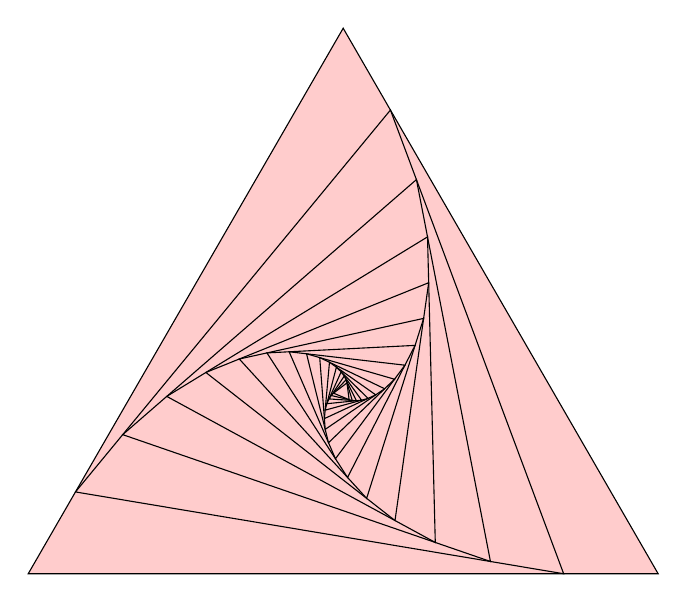
\begin{tikzpicture}
    \path[coordinate] (0,0)  coordinate(A)
                ++( 60:8cm) coordinate(B)
                ++(-60:8cm) coordinate(C);
    \draw[fill=red!20] (A) -- (B) -- (C) -- cycle;
    \foreach \x in {1,...,15}{%
        \path[coordinate] coordinate(X) at (A){};
        \path[coordinate] (A) -- (B) coordinate[pos=.15](A)
                            -- (C) coordinate[pos=.15](B)
                            -- (X) coordinate[pos=.15](C);
        \draw[fill=red!20] (A)--(B)--(C)--cycle;
    }
\end{tikzpicture}

}
\end{center}
\caption{PHEV Battery Charge Management Scenario}
\label{fig:scenario}
%\end{changemargin}
\end{figure}

\begin{itemize}

\item The scenario consists of one PHEV with a single user that makes predictable journeys between home and work during the weekdays and one trip to the shops on the weekend.

\item Charging and discharging has a fixed (but different) rate of flow and may take several hours to achieve.

\item There are charge points at all destinations and the PHEV has the choice of charging from the electricity grid or from a renewable source (wind or solar) where available. The choice of renewable for charging depends on the available output from the renewable source that has a predictable diurnal pattern.

\item There are discharge points at each location where the battery may supply power to the local grid circuit, but it cannot supply power to the feed-in circuit for the renewable source that has a separate meter and associated tariff.

\item A commenced charge/discharge operation may fail due to a user access, for instance when accessing the PHEV for a commute.

\item The PHEV is billed for charging (Consumption tariff) and credited for supplying energy (Feed-in tariff). Different rates apply for different locations. Feed-in tariff is always higher than Consumption tariff at every location.

\item Connection/disconnection to/from charge/discharge points at each location are considered separate procedures due to differences in the physical location of the points in relation to the parked PHEV.

\item The PHEV is fitted with a wireless receiver that is used by the network to send supply requests as well as demand data.



\end{itemize}

The goals of the MSA are to \footnote{There is no requirement to address peak network load for the initial system. This may be introduced later to experiment with multiple MSAs.}
:
\begin{enumerate}
\item[$G1$] Ensure that the PHEV has sufficient charge for all planned trips and any unplanned trips (limit N kms daily) by managing the battery charge and discharge cycles.
\item[$G2$] Optimise the PHEV running cost by considering the Feed-in and Consumption Tariffs at various locations.
\end{enumerate}

Within the BDI framework, achieving the MSA goals is reduced to making the correct plan choices in different context conditions. We choose to \emph{learn} such plan context conditions (for which purpose we will use decision trees). 

To understand how the MSA utilises the plan library consider the following context. \emph{The PHEV is parked at the office on a windy Monday morning and has an available charge of $095$. The local network broadcasts a power supply request.} The MSA must now deliberate and choose the best course of action.

Since the Feed-In Tariff is greater than the Consumption Tariff at the Office, then it is in the interest of the PHEV (goal G2) to entertain the request as long as it does not jeopardise the drive Home (goal G1). Even then, several strategies may be considered. Given enough time before close of business the PHEV may discharge beyond the critical threshold for $G1$ but then recharge again just in time to make the journey Home. Or it may play it safe and discharge only so that there is sufficient charge for the drive Home where it can recharge overnight. That decision in turn may depend on the difference between the Consumption Tariffs at the Office and at Home. 

\begin{figure}[htbp]
%\begin{changemargin}{-1.7in}{-1.7in}
\begin{center}
\fbox{
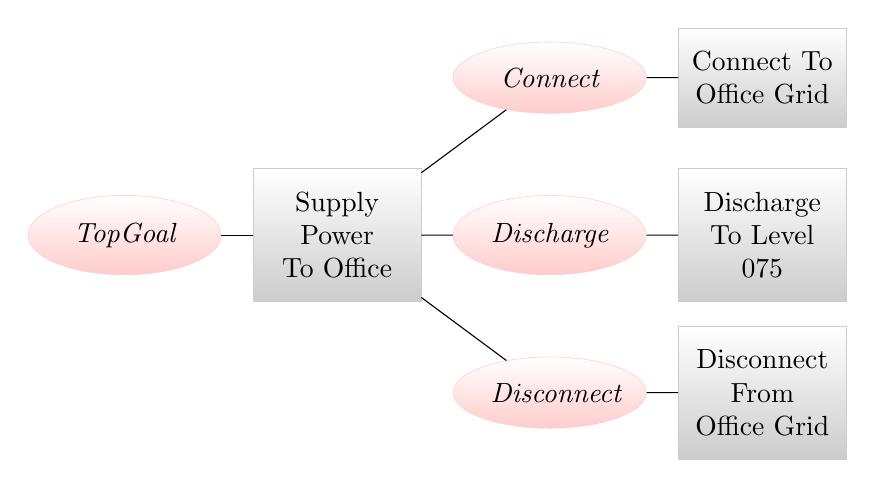
\begin{tikzpicture}
[
level distance=27mm, 
level 1/.style={sibling distance=20mm}, 
level 2/.style={sibling distance=20mm}, 
level 3/.style={sibling distance=20mm},
goal/.style={ellipse, very thin, draw=red!20, top color=white, bottom color=red!20, inner ysep=2mm, text width=15mm, text centered, font=\itshape},
plan/.style={rectangle, very thin, draw= black!20, top color=white, bottom color=black!20, inner ysep=3mm, text width=19mm, text centered}
] 
\node[goal] at (0,0) {TopGoal} [grow=right]
	child {node[plan] {Supply Power To Office}
		child {node[goal] {Disconnect}
			child {node[plan] {Disconnect From Office Grid}}
		}
		child {node[goal] {Discharge}
			child {node[plan] {Discharge To Level 075}}
		}
		child {node[goal] {Connect}
			child {node[plan] {Connect To Office Grid}}
		}
}; 
\end{tikzpicture}

}
\end{center}
\caption{Possible Goal/Plan Choice for a Supply Request at the Office}
\label{fig:plan-choice}
%\end{changemargin}
\end{figure}

Figure \ref{fig:plan-choice} shows one of many possible outcomes of the deliberation process in this context. Over time the MSA will explore different applicable choices in different situations and slowly converge to the optimal strategies.

The scenario offers several features that are interesting from a BDI-learning research perspective:

\begin{itemize}

\item Goal dependence. Both goals $G1$ and $G2$ are required for success and must be balanced equally by the MSA. Focussing on optimising one alone may lead to failure in the other. 

\item Failure recovery. In BDI agents the inherent failure recovery execution cycle may lead to plan failures, re-deliberation, and subsequent plan choices that succeed. This process results in seamless action sequences that represent the concatenation of several plan choices, some of which in fact led to failures. Such action sequences pose a challenge for the learning task as it becomes difficult to assign credit for failure and success to the correct sub-sequences.

\item Cost of failure. The scenario may be easily extended to include cost of failure in the decision making. For instance, failing to supply power to the network may not be as costly as failing to charge sufficiently for the drive home. Cost of failure makes the learning task more difficult as the agent can no longer explore (and therefore potentially fail) all available options equally.

\item Adaptation. The PHEV battery chemistry may change over time so the agent must continually tune its charge/discharge cycles to match the battery performance. This motivates the decision to learn plan context conditions in this scenario as opposed to encoding them at design time (using provided battery performance specifications).

\end{itemize}

\section {Mobile Storage Agent Design}

Figure \ref{fig:gptree} shows a possible BDI Goal/Plan Hierarchy for the MSA for achieving its goals. 

\begin{figure}[htbp]
\begin{changemargin}{-1.7in}{-1.7in}
\begin{center}
\fbox{
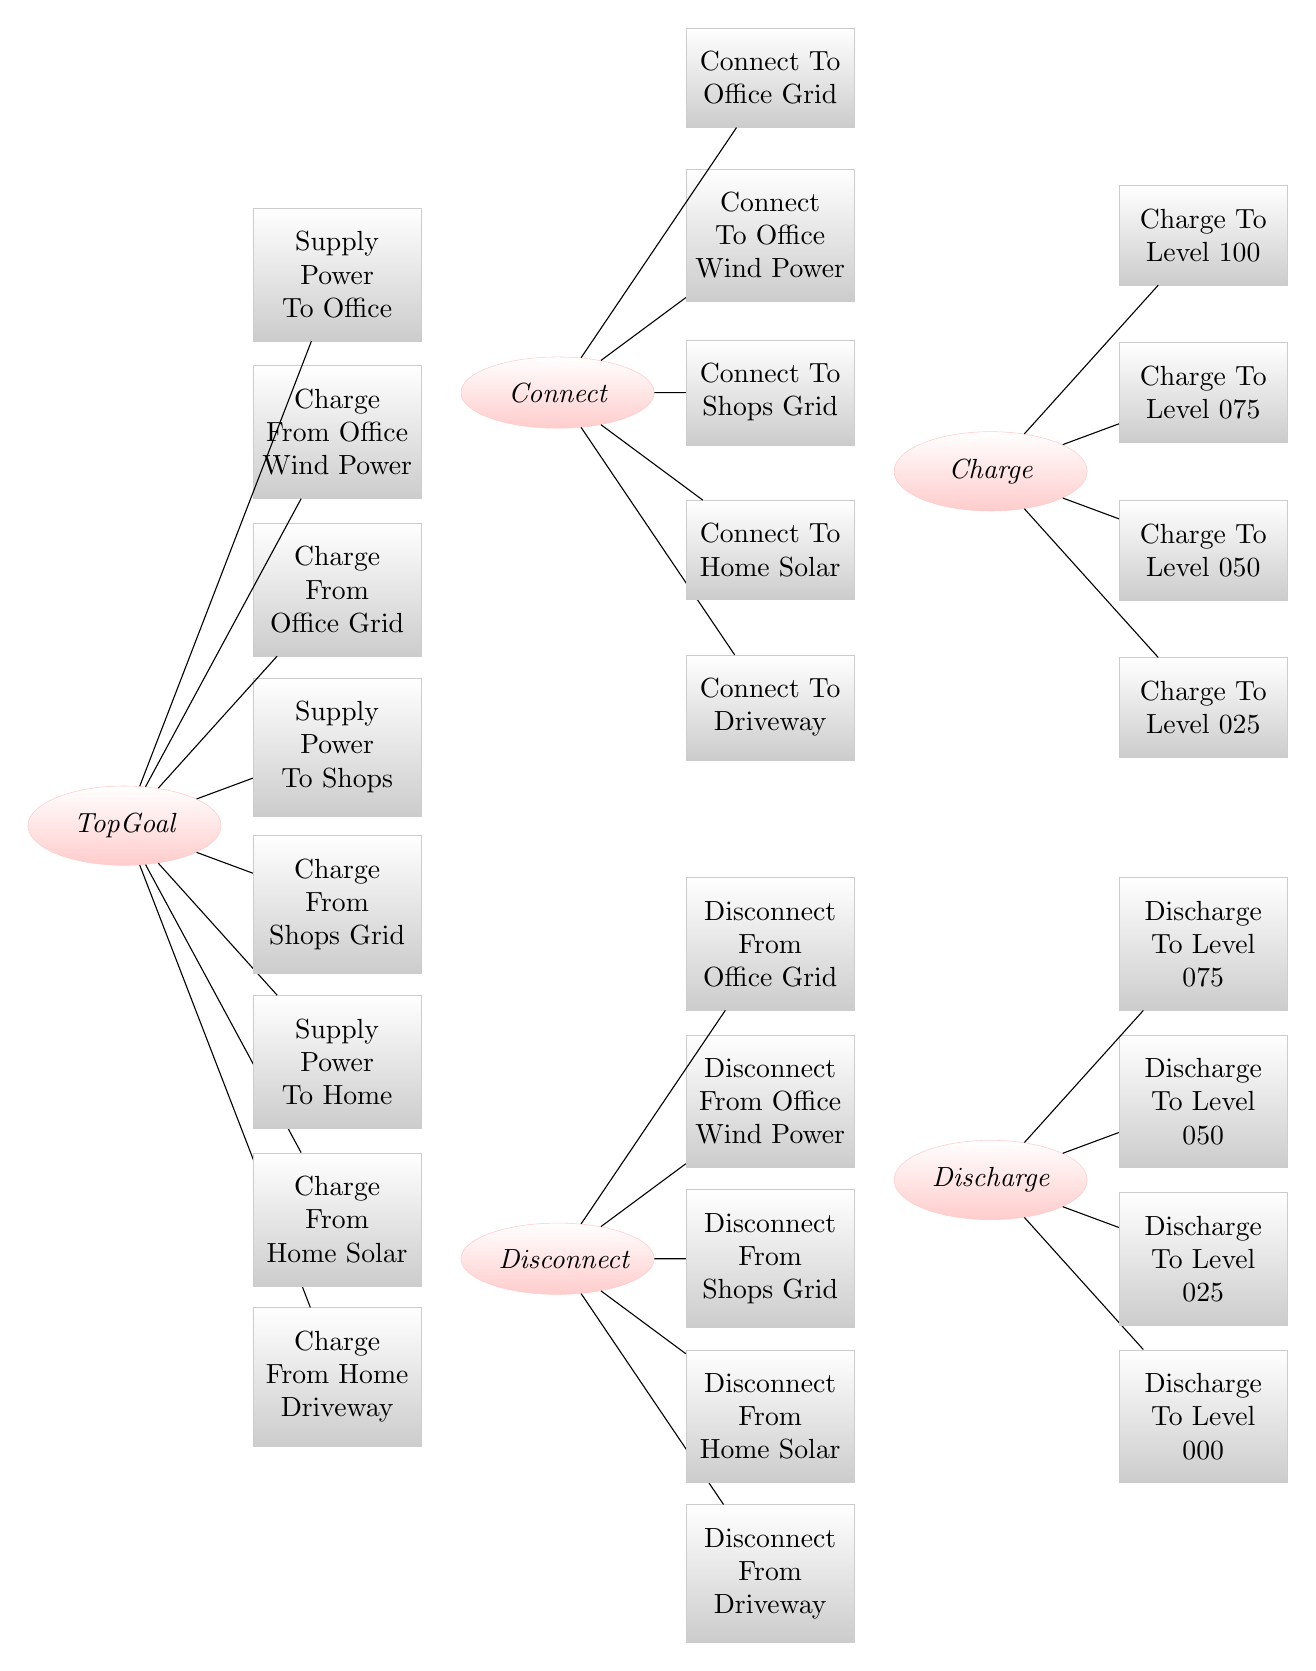
\begin{tikzpicture}
[
level distance=27mm, 
level 1/.style={sibling distance=20mm}, 
level 2/.style={sibling distance=12mm}, 
level 3/.style={sibling distance=12mm},
goal/.style={ellipse, very thin, draw=red!20, top color=white, bottom color=red!20, inner ysep=2mm, text width=15mm, text centered, font=\itshape},
plan/.style={rectangle, very thin, draw= black!20, top color=white, bottom color=black!20, inner ysep=3mm, text width=19mm, text centered}
] 
\node[goal] at (0,0) {TopGoal} [grow=right]
	child {node[plan] {Charge From Home Driveway}}
	child {node[plan] {Charge From Home Solar}}
	child {node[plan] {Supply Power To Home}} 
	child {node[plan] {Charge From Shops Grid}}
	child {node[plan] {Supply Power To Shops}}
	child {node[plan] {Charge From Office Grid}}
	child {node[plan] {Charge From Office Wind Power}}
	child {node[plan] {Supply Power To Office}
}; 
\node[goal]  at (5.5,5.5) {Connect} [grow=right]
	child {node[plan] {Connect To Driveway}}
	child {node[plan] {Connect To Home Solar}}
	child {node[plan] {Connect To Shops Grid}}
	child {node[plan] {Connect To Office Wind Power}}
	child {node[plan] {Connect To Office Grid}
};

\node[goal]  at (11,4.5) {Charge} [grow=right]
	child {node[plan] {Charge To Level 025}}
	child {node[plan] {Charge To Level 050}}
	child {node[plan] {Charge To Level 075}}
	child {node[plan] {Charge To Level 100}
};

\node[goal]  at (11,-4.5) {Discharge} [grow=right]
	child {node[plan] {Discharge To Level 000}}
	child {node[plan] {Discharge To Level 025}}
	child {node[plan] {Discharge To Level 050}}
	child {node[plan] {Discharge To Level 075}
};

\node[goal]  at (5.5,-5.5) {Disconnect} [grow=right]
	child {node[plan] {Disconnect From Driveway}}
	child {node[plan] {Disconnect From Home Solar}}
	child {node[plan] {Disconnect From Shops Grid}}
	child {node[plan] {Disconnect From Office Wind Power}}
	child {node[plan] {Disconnect From Office Grid}
};
\end{tikzpicture}

}
\end{center}
\caption{BDI Goal-Plan Hierarchy for the MSA}
\label{fig:gptree}
\end{changemargin}
\end{figure}


\bibliographystyle{plain}
\bibliography{msa.bib} 

\end{document}